\chapter{概念教学}

\section{概念}
\begin{multicols}{2}
\subsection{数学概念}
根据 $R$ (如 $x_1, x_2, \ldots, x_n$ 是否有运算)将数学概念分为:
\begin{itemize}
    \item 运算性概念。
    \begin{itemize}
        \item 程序性概念
        \item 构造性概念
    \end{itemize}
    \item 陈述性概念。
\end{itemize}
运算性概念:\\
是名需要构造出一个满足某种属性的对象后再运算的概念。
\columnbreak
\subsection{特征表说}
概念/概念的表征:
\begin{enumerate}
    \item 定义性特征:一类个体事物具有的共同属性(记 $x_1, x_2, \ldots, x_n$)。
    \item 定义性特征之间的关系:整合定义性特征的规则(记 $R$)。
\end{enumerate}

\subsection{概念的分类}
维果斯基将概念分为:
\begin{itemize}
    \item \textbf{日常概念}:未经过专门的教学,人们通过日常生活的经验积累既能掌握的概念。
    \item \textbf{科学概念}:在教学过程中通过揭示概念内涵而形成的概念。
\end{itemize}
\end{multicols}
\begin{multicols}{2}
\subsection*{陈述性概念习得过程}
\begin{itemize}
    \item 学:激活 $\rightarrow$ 精致 $\rightarrow$ 检验 $\rightarrow$ 形成图式。
    \item 教:
    \begin{itemize}
        \item 激活
        \begin{itemize}
            \item 复习 $x$ 及 $R$
        \end{itemize}
        \item 精致
        \begin{itemize}
            \item 给出 $x$ 与 $R$ 的例子,要求学生概括内涵
        \end{itemize}
        \item 检验
        \begin{itemize}
            \item 给出正反例,要求学生判断
        \end{itemize}
        \item 形成图式
        \begin{itemize}
            \item 多角度提示概念本质。
            \item 与相关概念的联系。 
        \end{itemize}
    \end{itemize}
\end{itemize}
\columnbreak
\subsection*{运算性概念习得过程}
\begin{enumerate}
    \item \textbf{数学概念二重性 —— 过程和对象}:
    \begin{itemize}
        \item 过程——含操作(运算程序)。
        \item 对象——指数学概念的定义结构或关系。
    \end{itemize}
    \item \textbf{学生容易形成数学对象的过程,而难以形成数学对象的结构}。
    \item \textbf{课例:“分数”的概念教学}:\\
    具体情境中的分数概念,对
    \begin{itemize}
        \item 面积模型。
        \item 线段模型:进行平均分表示出整体中的某个部分。
        \item 离散模型。
    \end{itemize}
\end{enumerate}
\end{multicols}

\section{数学概念教学的几种模式}

\subsection{概念形成模式}

\begin{figure}[H]
    \centering
    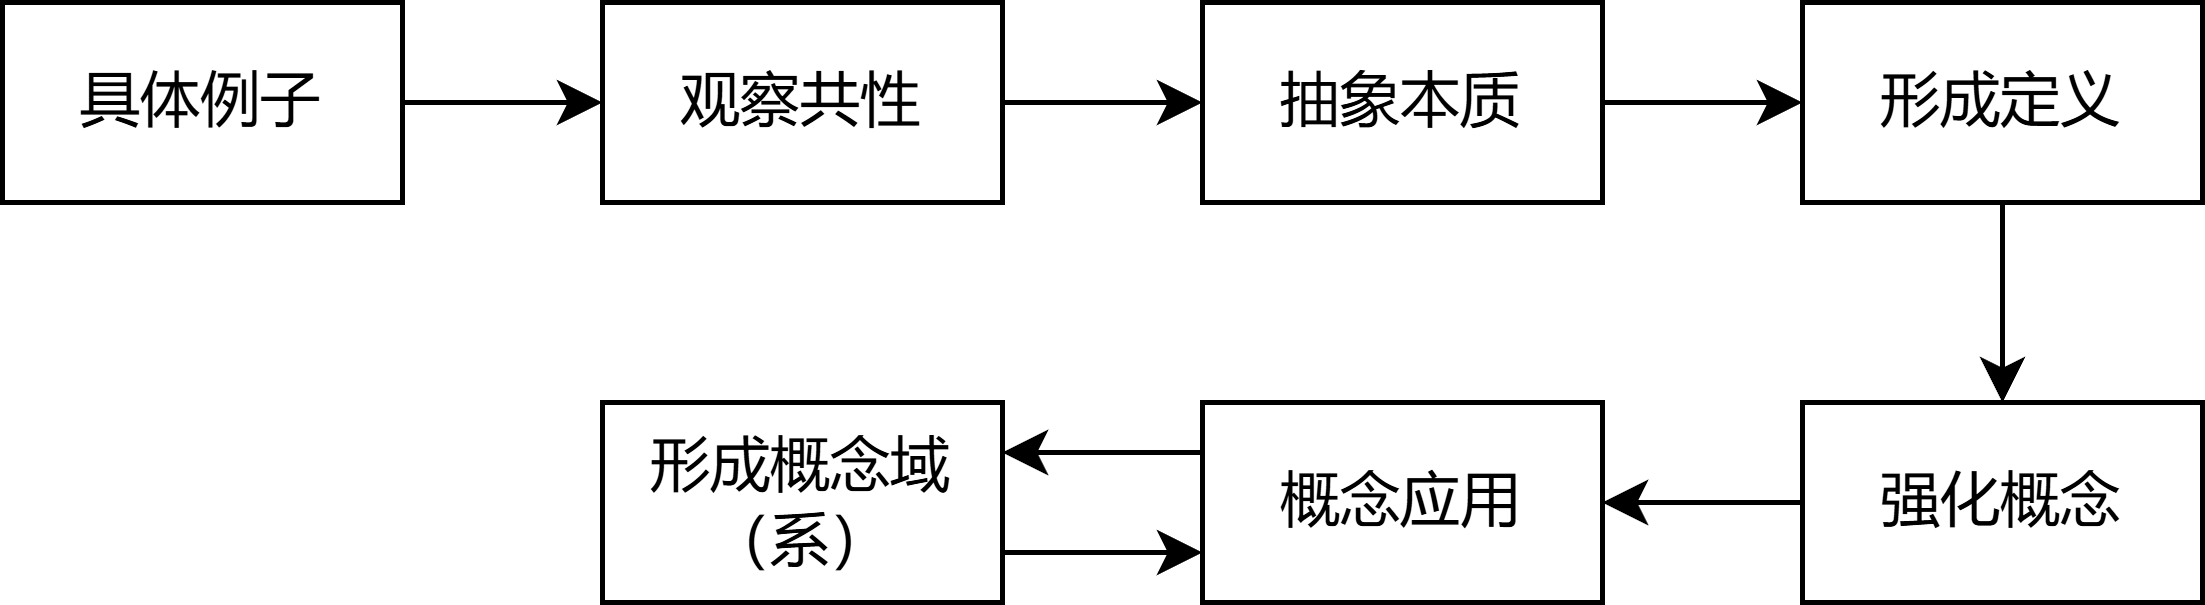
\includegraphics[width=0.5\linewidth]{image/概念形成模式.png}
\end{figure}

\subsection{概念同化模式}

\begin{figure}[H]
    \centering
    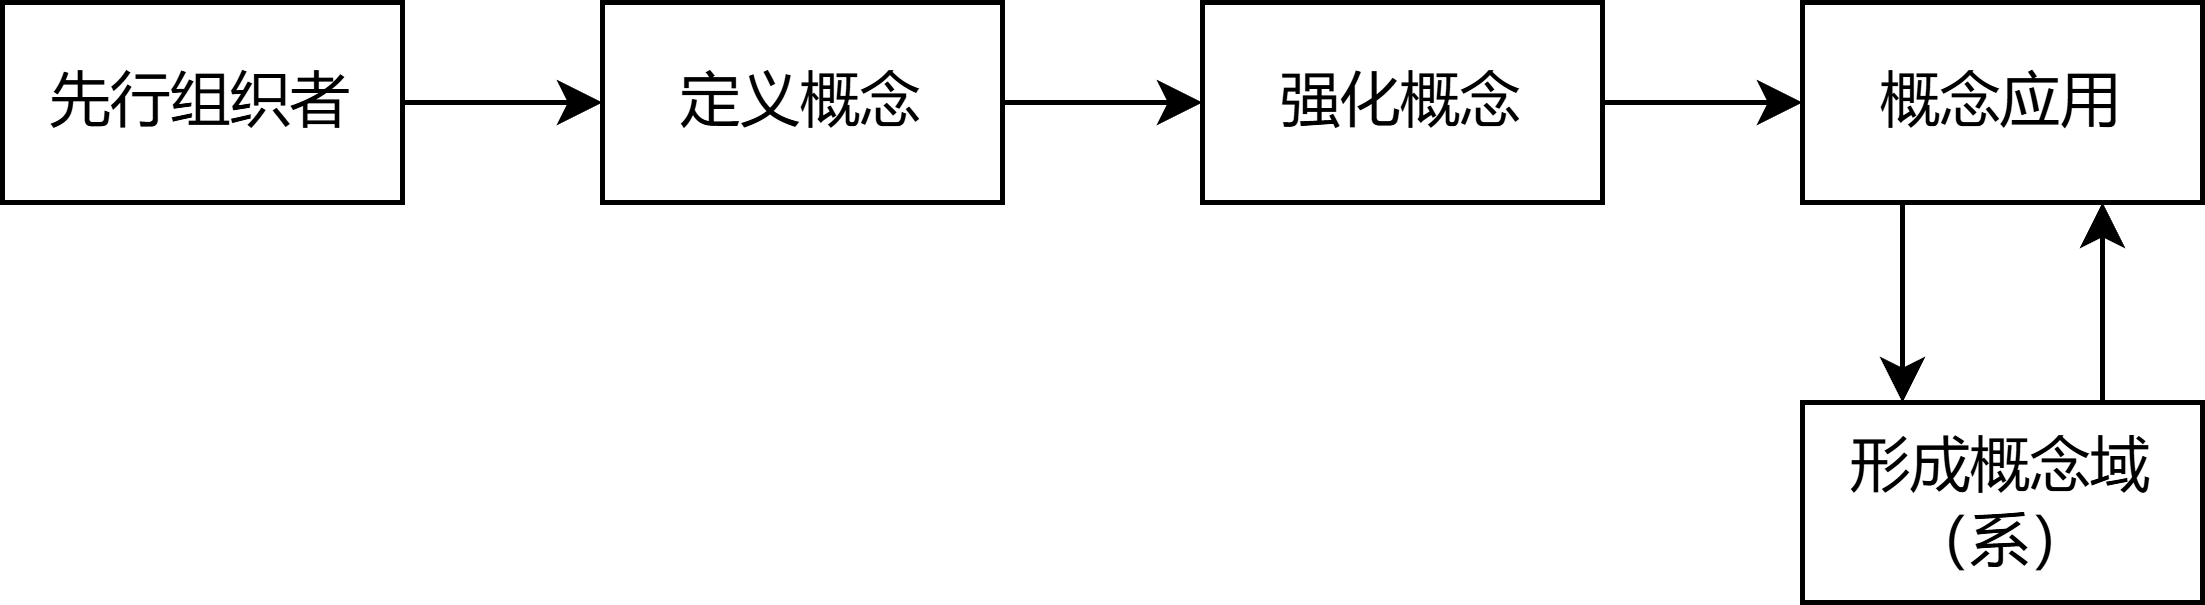
\includegraphics[width=0.5\linewidth]{image/概念同化模式.png}
\end{figure}

\subsection{问题引申模式}

\begin{figure}[H]
    \centering
    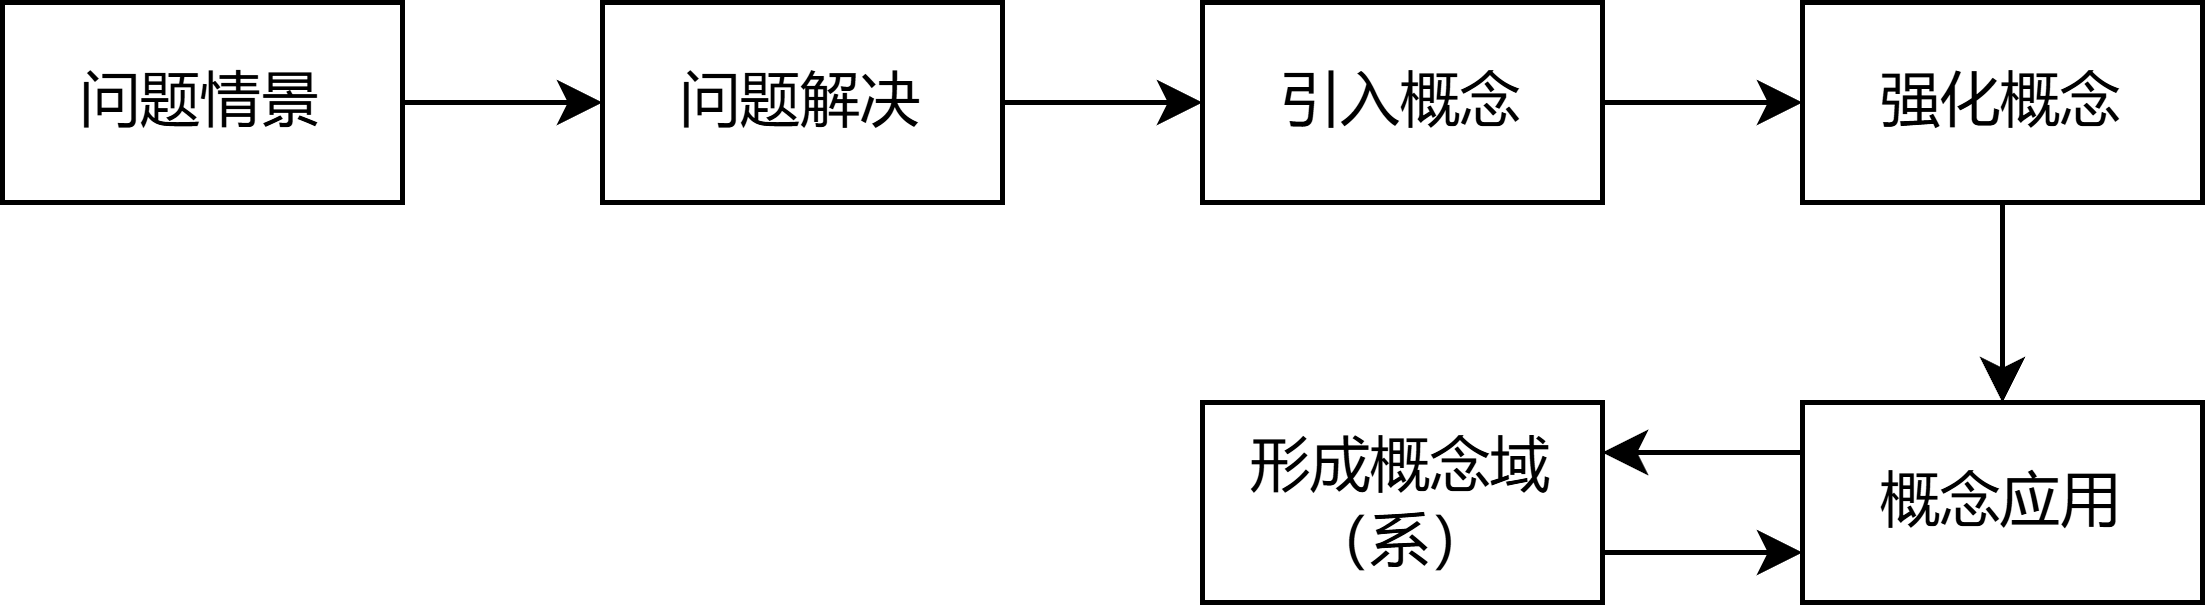
\includegraphics[width=0.5\linewidth]{image/问题引申模式.png}
\end{figure}

\section{数学概念教学的两个策略}

\subsection{正反例强化策略}
\begin{multicols}{2}
    

\textbf{正反例构建 —— 美林-丁尼森模式}

前提概念:若对于 $C = R(x_1, x_2, \ldots, x_n)$

\begin{itemize}
    \item 相关属性:$x_1, x_2, \ldots, x_n$
    \item 无关系性:与概念本质属性无关,但会伴随概念原型出现的属性。
\end{itemize}

\columnbreak

\textbf{正反例特征与效果}:
\begin{itemize}
    \item 按例子的特征来呈现正反例的效果最好。
    \item 好的正反例应具有3个特征:\\
    1. 相互匹配。
    2. 差异大。
    3. 由简单到困难。
    \item 正例数量>=反例数量,课堂教学1:1。
\end{itemize}
\end{multicols}

\begin{table}[h!]
\centering
\begin{tabular}{c|c|c|c}
  & 属性 & 值1 & 值0 \\ 
\hline
\multirow{2}{*}{相关} 
& 未知数 & 含 & 不含 \\ \cline{2-4}
& 等式 & 是 & 不是 \\ 
\hline
\multirow{3}{*}{无关} 
& 未知数个数 & 1个 & >=2个 \\ \cline{2-4}
& 未知数位置 & 左/右 & 左+右 \\ \cline{2-4}
& 未知数的形式 & 字母 & 非字母 \\ 
\hline
\end{tabular}
\caption{方程的正反例构造}
\end{table}

\subsection{完善 CPFS 结构的教学策略}

\begin{multicols}{2}
    

\begin{enumerate}
    \item \textbf{注重从多角度揭示概念的内涵}:
    \begin{itemize}
        \item 多种情境(多种特例)。
        \item 多重层次(数学概念发展性)。
        \item 不同侧面(定义一个概念可选不同特征)。
        \item 不同结构(从不同结构中刻画)。
    \end{itemize}
\columnbreak
    \item \textbf{形成概念体系}:
    \begin{itemize}
        \item 建立概念网络。
        \item 明示概念之间的关系。
        \item 揭示在这个概念体系中的数学思想方法。
    \end{itemize}

    \item \textbf{加强概念的应用}:
    \begin{itemize}
        \item 低层次——知觉水平的应用:能判断一组特例是否属于某个概念的范畴。
        \item 高层次——思维水平的应用:将概念用于问题解决中。
    \end{itemize}
\end{enumerate}
\end{multicols}